\documentclass[10pt,handout]{beamer}

\usepackage[french]{babel}
\usepackage[T1]{fontenc}
\usepackage[utf8]{inputenc}
\usepackage[
    left = \flqq{},%
    right = \frqq{},%
    leftsub = \flq{},%
    rightsub = \frq{} %
]{dirtytalk} 	% for \say{}
\usepackage{xcolor} 	% for color text
\usepackage{csquotes}
\usepackage{amssymb}
\usepackage{mathtools}
\usepackage{array}

\usetheme{Frankfurt}
\usetheme{CambridgeUS}
\usetheme{JuanLesPins}
%\usetheme{Montpellier}
%\usetheme{Madrid}

\usecolortheme{dolphin}

\useinnertheme{circles}
\usefonttheme{structurebold}
\useoutertheme{default}

%\hypersetup{pdfpagemode=FullScreen}

\title[Moteur de requêtes SQL]{Implémentation d’un moteur de \\ requêtes SQL simples}
\author[Bouzidi, Elhouiti, Kezzoul, Zeroual, Feï]{Bouzidi Belkacem - Elhouiti Chakib \\ Kezzoul Massili - Zeroual Ramzi \\ Feï Yang}
\institute[]{Université de Montpellier}
\date{\today}

% Pour inserer une frame de sommaire avant chaque debut de section
\AtBeginSection[]
{
  \begin{frame}
    \tableofcontents[hideothersubsections,currentsection,subsectionstyle=show/shaded/hide]
  \end{frame}
}

% Mettre les listes en triangle
\setbeamertemplate{itemize item}[triangle]

%Insertion d'un logo
\newif\ifplacelogo % create a new conditional
\placelogotrue % set it to true
\logo{\ifplacelogo
\includegraphics[height=12mm]{img/univ-montpellier.png}\fi}

%------------------------------------------------------%
% page de titre
%------------------------------------------------------%
\begin{document}

\placelogofalse
\begin{frame}
	\titlepage
\end{frame}

\placelogotrue

%------------------------------------------------------%
% Tables des matières
%------------------------------------------------------%

\begin{frame}{table}
	\frametitle{Sommaire}
	\tableofcontents
\end{frame}

%------------------------------------------------------%
% Intro
%------------------------------------------------------%
\section{Introduction}
\begin{frame}{Introduction}{Presentation du projet}
\begin{itemize}
  \item Projet choisi : conception et développement d’un moteur d’évaluation de requêtes SQL en mémoire vive.
  \item Forme des requêtes :
  \begin{itemize}
    \item SELECT : Projection
    \item FROM : Jointure
    \item WHERE : Selection
  \end{itemize}
  \item Fichiers pris en charge : un ou plusieurs fichiers CSV
  \begin{itemize}
    \item Un fichier CSV est un fichier texte
    \item Une Ligne du texte correspond à une ligne du tableau
    \item Les virgules correspondent aux séparations entre les colonnes
  \end{itemize}
\end{itemize}
\end{frame}

\begin{frame}{Introduction}{Organisation}
  \begin{itemize}
    \item Réunions :
    \begin{itemize}
      \item Etudiants : trois à quatre fois par semaine
      \item Encadrante : une fois par semaine
    \end{itemize}
    \item Decoupage du projet :
    \begin{itemize}
      \item Phase de modélisation
      \item Phase de développement
      \item Finalisation du projet
    \end{itemize}
    \item Outils de collaboration : GitLab
  \end{itemize}
\end{frame}

\subsection{Organisation du projet}

\begin{frame}{Organisation}

\end{frame}

\placelogofalse
\begin{frame}{Objectif de l'application}
  \makebox[\textwidth]{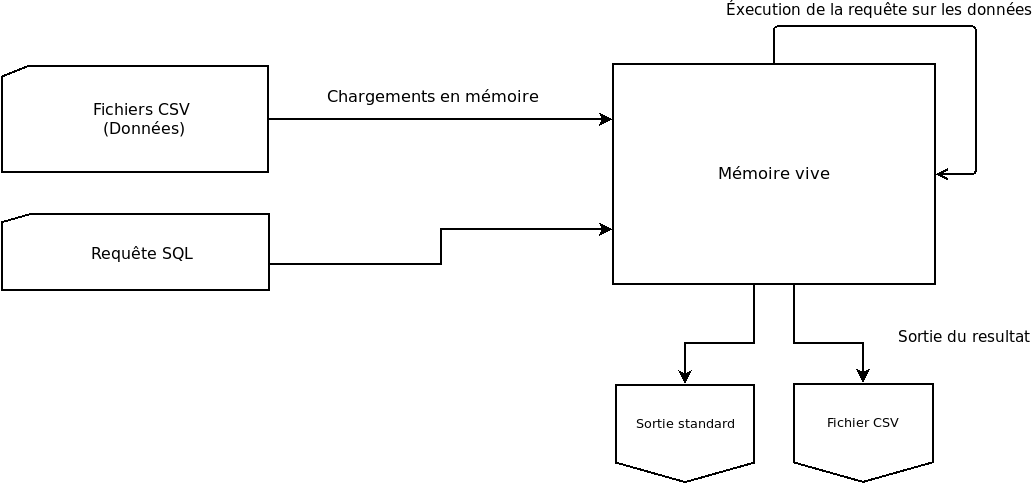
\includegraphics[width=\paperwidth]{img/role_prog.png}}
\end{frame}
\placelogotrue

\subsection{Présentation du SQL et des bases de données}
\begin{frame}{Présentation}{SQL et les bases de données}
  \begin{block}{Base de données}
    Une base de données (en anglais database), permet de stocker et de manipuler des données brutes ou d'informations.
  \end{block}

  \begin{block}{Système de gestion de base de données}
    Un SGBD est un logiciel système servant à stocker, à manipuler ou gérer, et à partager des informations dans une base de données, en garantissant la qualité, la pérennité et la confidentialité des informations, tout en cachant la complexité des opérations.
  \end{block}

  SGBD les plus utilisés :
    \begin{itemize}
      \item Oracle Database
      \item MySQL
      \item ...
    \end{itemize}
  
\end{frame}

\begin{frame}{Structered Query Languages}
  \begin{block}{Intérpreteur de requêtes SQL}
    Le SQL est un langage informatique normalisé servant à exploiter des bases de données relationnelles.
  \end{block}

  Les requêtes SQL considéré par notre programme sont sous cette forme :
  
  \begin{block}
    
    \textit{SELECT nomAttribut1,...,nomAttribut2 \\ FROM nomTable1,..., nomTable2 \\ WHERE nomAttributX = nomAttributY OR ... AND nomAttributZ = ZZ}
  \end{block}

\end{frame}

%------------------------------------------------------%
% Modélisation
%------------------------------------------------------%

\section{Modélisation}

\begin{frame}{Modélisation}

\end{frame}

\begin{frame}{Structure des données}
  \makebox[\textwidth]{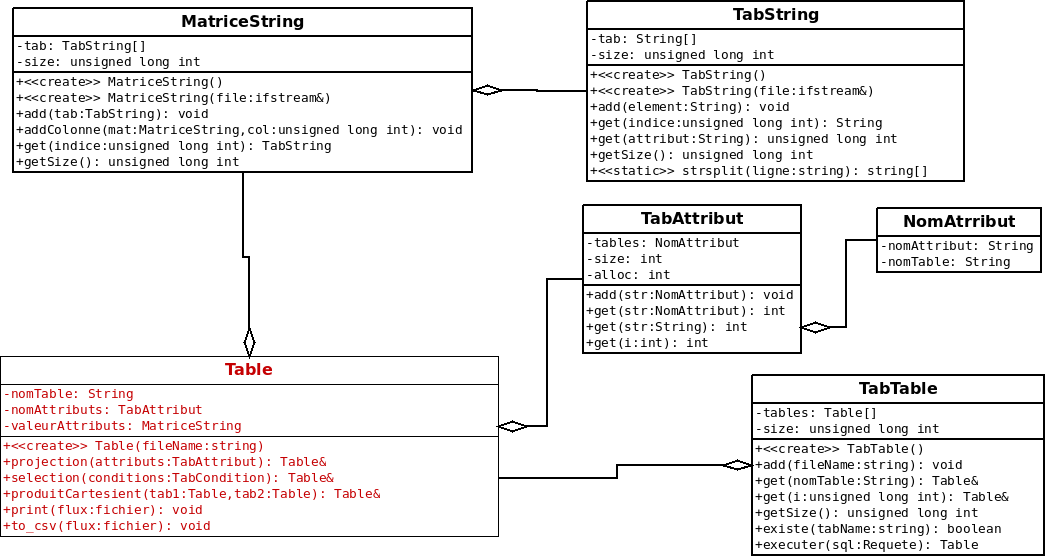
\includegraphics[width=\paperwidth]{img/sql.png}}
\end{frame}

\begin{frame}{Structure de la requête}
  \makebox[\textwidth]{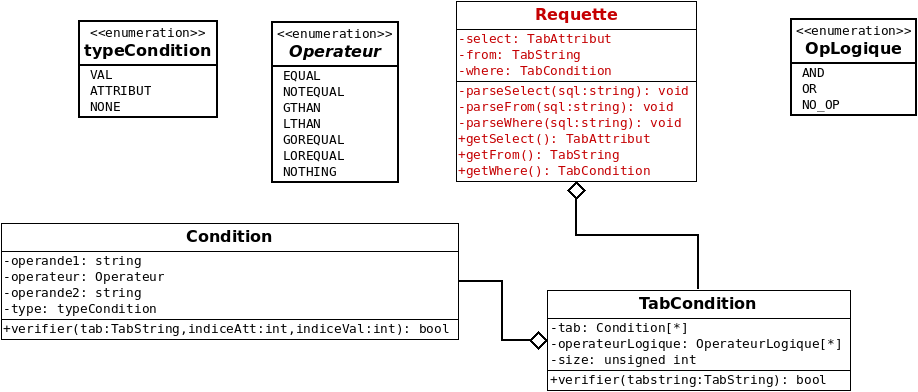
\includegraphics[width=\paperwidth]{img/requette.png}}
\end{frame}

%------------------------------------------------------%
% Implémentation
%------------------------------------------------------%
\section{Implémentation}

\begin{frame}{Implémentation}
  Les grandes lignes de l'implémentation : 
  \begin{itemize}
    \item Choix du C++ comme langage de programmation,
    \item Répartition du développement en trois parties principales :
    \begin{itemize}
      \item Chargement des données,
      \item Intérpretationet éxecution de la requête,
      \item Restitution des données.
    \end{itemize}
    \item Utilisation du programme,
    \item Phases de tests.
  \end{itemize}
\end{frame}

\begin{frame}{Développement}{Chargement des données}
  \begin{itemize}
    \item Implémentation des classes,
    \item Interpréter un fichier CSV,
    \item Fonction strsplit,
    \item Parser toutes les lignes du fichiers CSV,
  \end{itemize}
\end{frame}

\begin{frame}{Développement}{La requête}
  \begin{block}{Intérpretation}
    Nous nous sommes occupés à trouver une manière de découper la requête afin de stocker chaque partie dans l’attribut correspondant.
  \end{block}
  
  \begin{block}{Éxecution}
    Notre application exécute la requête en trois étapes consécutives et complémentaires pour effectuer le traitement nécessaire.
    \begin{itemize}
      \item Le produit cartésien,
      \item La selection,
      \item La projection.
    \end{itemize}
  \end{block}
\end{frame}

%------------------------------------------------------%
% Démonstration
%------------------------------------------------------%

\section{Démonstration}

%------------------------------------------------------%
% Conclusion
%------------------------------------------------------%

\section{Conclusion}

\begin{frame}{Bilan}

\end{frame}

\begin{frame}{Perspective}

\end{frame}

\end{document}
